Here we present the estimation of $\beta$ given corresponding values of $\alpha$, as visualized in Figures \ref{fig:tiling_time_comparison_extra_alphas} and \ref{fig:tiling_comparison_extra_alphas}. The calculation method is described in Appendix \ref{appendix:k_set_coverage_analysis}. We computed the values for $\beta$ in Table \ref{table:beta_alpha_dependency} based on the data from Figure \ref{fig:tiling_comparison_extra_alphas}.

\begin{figure}[htb]
      \captionsetup{
                   skip=-2pt
                 }
  \begin{center}
    \begin{subfigure}{.49\textwidth}
      \captionsetup{
                   font={scriptsize},
                   skip=-5pt
                 }
      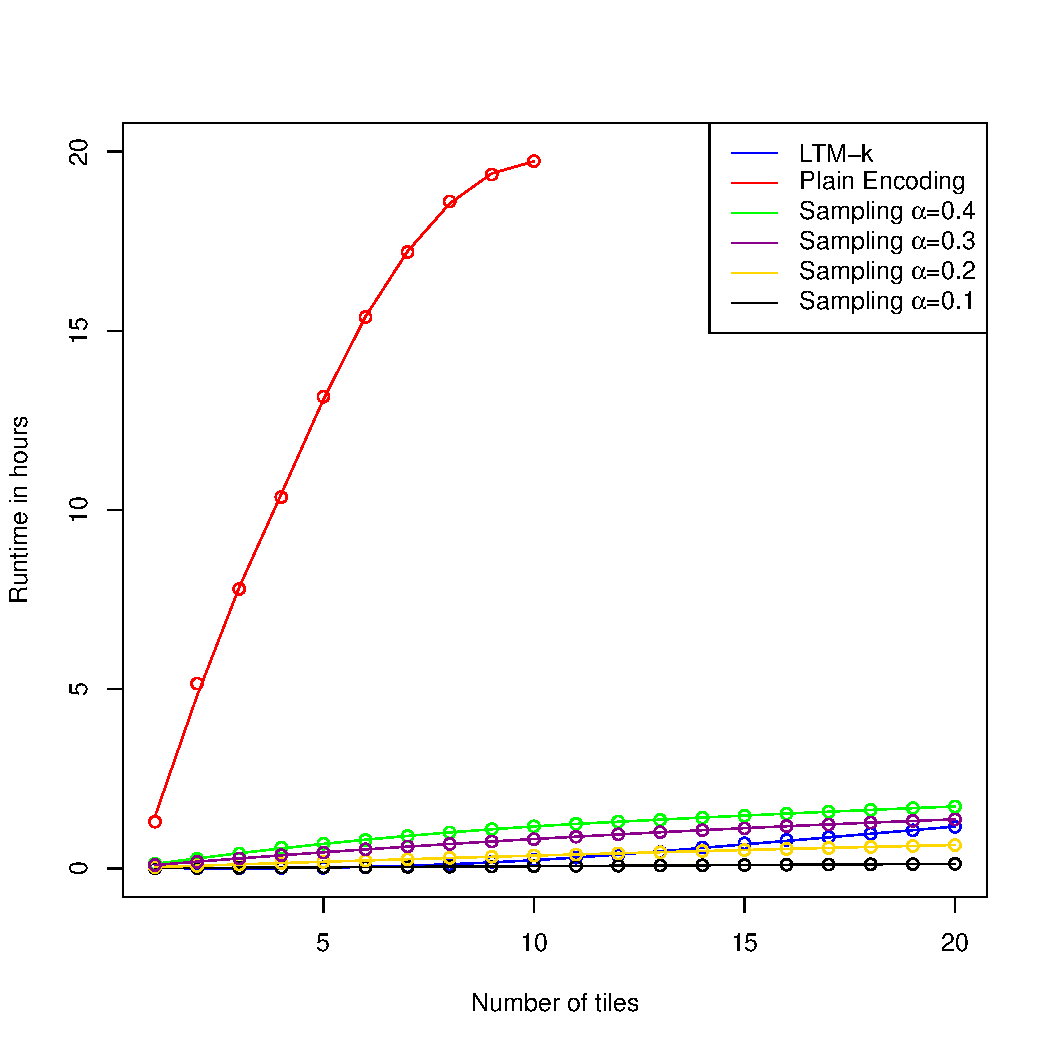
\includegraphics[width=\textwidth]{tiling-time-plot_extra_alphas.pdf}
      \caption{Runtime}
      \label{fig:tiling_time_comparison_extra_alphas}
    \end{subfigure}
    \hfill 
    \begin{subfigure}{.49\textwidth}
      \captionsetup{
                   font={scriptsize},
                   skip=-5pt
                 }
      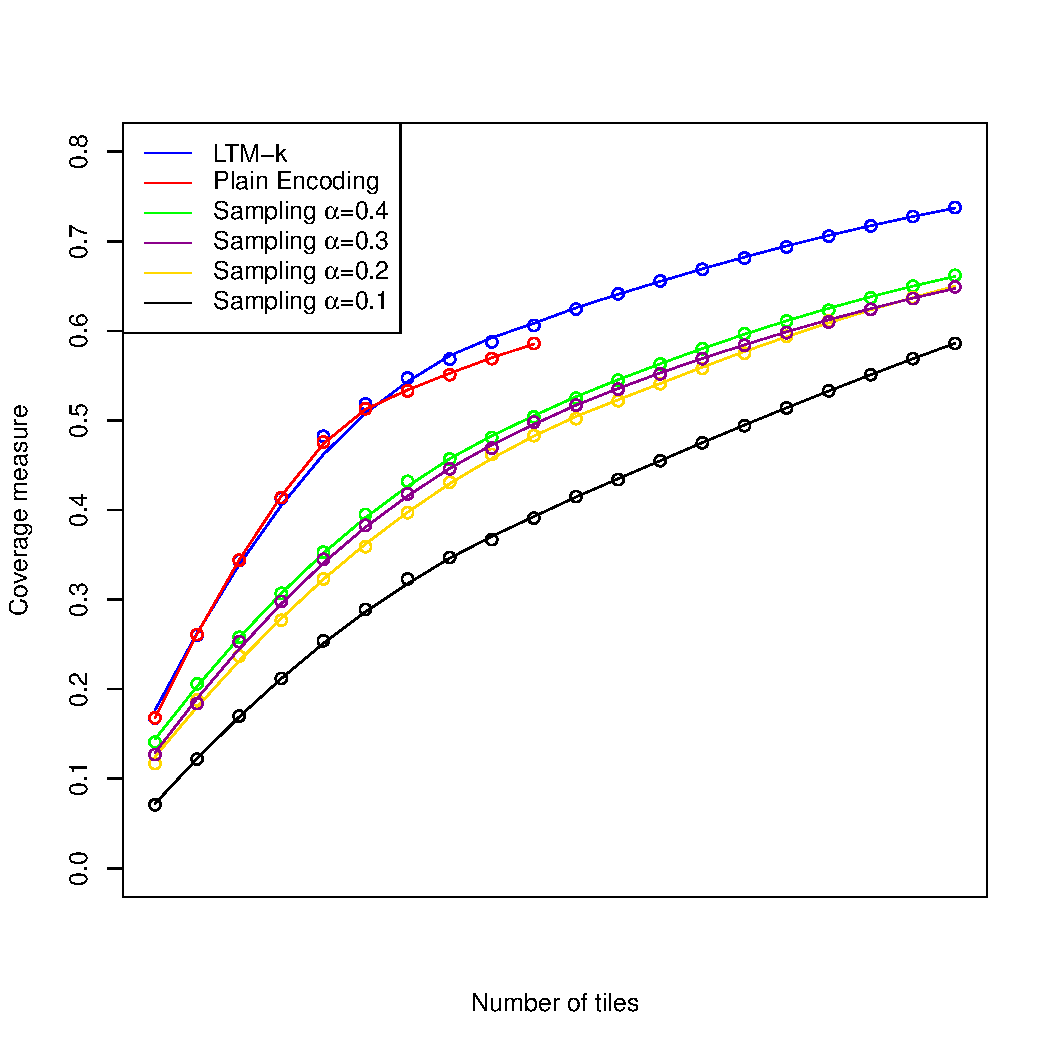
\includegraphics[width=\textwidth]{tiling_comparison_extra_alphas.pdf}
      \caption{Coverage}
      \label{fig:tiling_comparison_extra_alphas}
    \end{subfigure}
  \caption{Tiling comparison (runtime, coverage) with LTM-k (Mushroom dataset)}
  \end{center}
\end{figure}

\begin{table}[htb]
  \centering
  \caption{An empiricial reconstruction of $\beta$, given the values of $\alpha$}
  \label{table:beta_alpha_dependency}
  \begin{tabular}{l | c c c c}
    $\alpha$ & 0.1 & 0.2 & 0.3 & 0.4\\
    $\beta$ & 0.55& 0.73 & 0.76 & 0.79 
  \end{tabular}
\end{table}


